\documentclass{gescons}

\genre {Resumo do Biênio}
\author{Ana Claudia Prado e Magda Stapf Amancio}
\authorrole{Coordenadoras Editares -- Biênio 2024-2025}
\title{Editares Conquista a Certificação Institucional da UNICIN em 2024}

\begin{document}
    \makeentrevistatitle
    %\maketitle

    %\fullwidthimage{fields}{b}

    %\coverart{back/editorial}
    \coverart{../fundo-generico.png}
    
%    \begin{multicols}{2}

%\begin{center}
%    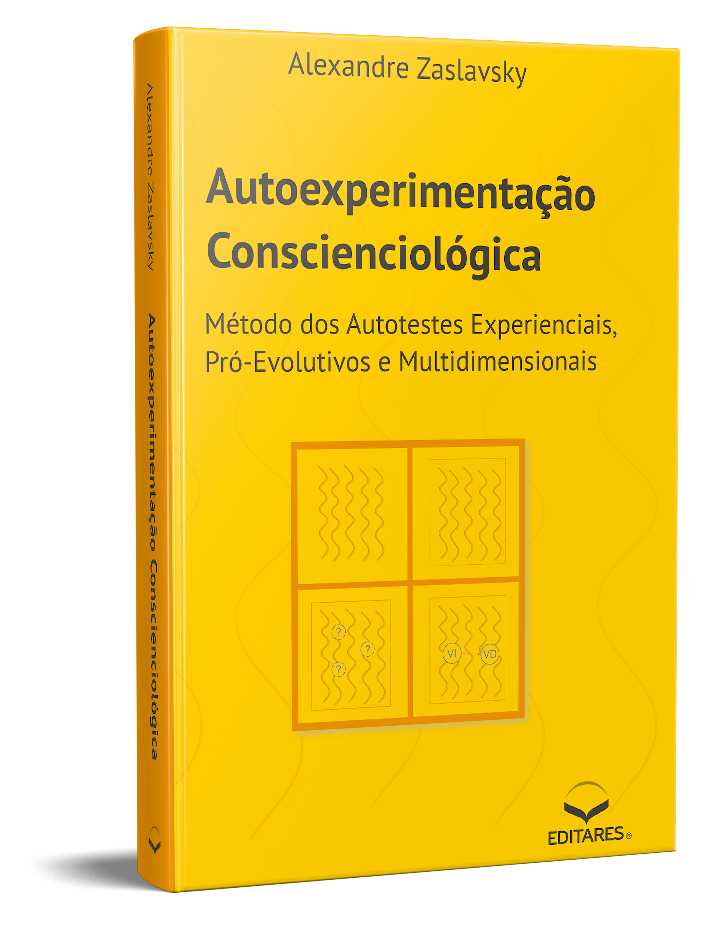
\includegraphics[width=4cm]{articles/entrevista/mockups/Alexandre-Zas.png}
%\end{center}


%\usepackage{graphicx}
%\usepackage{subcaption} % se quiser sublegendas

\begin{figure}[h]
  \centering
  \begin{subfigure}[b]{0.49\textwidth}
    \includegraphics[height=60mm,keepaspectratio]{articles/resumo/fotos/materia3/d94f6571-cf63-48d2-976b-507cbf8cafc5.jpg}
\end{subfigure}
\begin{subfigure}[b]{0.49\textwidth}
    \includegraphics[height=60mm,keepaspectratio]{articles/resumo/fotos/materia3/06eb15bb-01a3-43d5-84e2-67f62c13a53e.jpg}
  \end{subfigure}
\end{figure}


%\noindent\includegraphics[width=9cm, height=9cm]{articles/resumo/fotos/materia1/IMG20241023144802.jpg}

A Editares recebeu, pela segunda vez, a \emph{Certificação Institucional
da UNICIN,} após avaliação realizada em 2024. A primeira certificação
ocorreu em 2019. Esse reconhecimento reforça o alinhamento da IC à
maxiproéxis grupal da \emph{Comunidade Conscienciológica Cosmoética
Internacional} (CCCI) e ao compromisso contínuo com a
interassistencialidade tarística.

A \emph{Certificação Institucional} promovida pela UNICIN não tem
caráter técnico ou legal como as certificações normativas nacionais, mas
representa um \emph{aval grupal,} validando a atuação funcional e
interassistencial da IC dentro do fluxo da CCCI.

O processo é coordenado pelo \emph{Comitê Conscienciocêntrico da
UNICIN,} que envia um formulário-padrão às \emph{Instituições
Conscienciocêntricas} (ICs). As respostas são analisadas por conselhos
especializados:

\begin{itemize}
\item
  Conselho de Interassistência Jurídica da Conscienciologia (CIAJUC)
\item
  Conselho Intercientífico
\item
  Conselho de Parapedagogia
\item
  Conselho Intervoluntariado
\item
  Conselho de Interassistência em Economia, Finanças e Orientação Fiscal
  (CIEFFI)
\end{itemize}

A certificação visa verificar o grau de maturidade institucional em
aspectos como gestão, interassistência, parapedagogia, voluntariado e
sustentabilidade organizacional, sempre sob a ótica dos princípios
conscienciais.

A conquista da certificação pela Editares em 2024 reflete o esforço
coletivo dos voluntários e a consolidação do trabalho editorial
tarístico, contribuindo com a reurbex planetária e a expansão da
Conscienciologia.

Editares agradece à UNICIN e aos conselhos envolvidos pela seriedade no
processo, e renova seu compromisso com a interassistência tarística e o
fortalecimento da maxiproéxis grupal.


%v \textbf{{[}INSERIR UMA DAS FOTOS DA PASTA ``MATÉRIA 3''{]}}



%\noindent\includegraphics[width=9cm, height=9cm]{articles/resumo/fotos/materia1/IMG20241023143149.jpg}
        
%    \end{multicols}
\end{document}
